%\documentclass[t]{beamer}
\documentclass[aspectratio=169]{beamer}
\usepackage{helvet}
\usepackage{calc}
\usepackage[utf8]{inputenc}
\usepackage[english]{babel}

\usetheme{Ilmenau}

\setbeamercovered{transparent}
\setbeamertemplate{navigation symbols}{}

\usepackage{units}
\usepackage{amsbsy}
\usepackage{amsmath}
\usepackage{amssymb}
\usepackage{graphics}
\usepackage{graphicx}
\usepackage{epsf}
\usepackage{epsfig}
\usepackage{fixmath}
%\usepackage{pgfmath}
\usepackage{wrapfig}


\title{FOSDEM infrastructure review}
\subtitle{We have become so good, this is basically the talk from two years ago :)}
\author{Richard Hartmann,\\
RichiH@\{freenode,OFTC,IRCnet\},\\
richih@\{fosdem,debian\}.org}
\date{2020-02-02}


\begin{document}

% hide all subsections
\setcounter{tocdepth}{1}

\begin{frame}
	\titlepage
\end{frame}



%\begin{frame}
%	\frametitle{Statistics}
%	\tableofcontents
%\end{frame}

%\section{asdf}

\begin{frame}
	\frametitle{Repetition}
	\vfill
	\begin{itemize}
		\item This is almost the same talk as last year, and the year before that
		\item Which is good!
	\end{itemize}
	\vfill
\end{frame}

\begin{frame}
	\frametitle{Repetition}
	\begin{center}
		\vfill
		When I switched to doing infrastructure for FOSDEM around 2015, this was distilled pain
		\vfill
	\end{center}
\end{frame}

%\begin{frame}
%	\frametitle{IPv6 is here}
%	\vfill
%	\begin{itemize}
%		\item First year we had more IPv6-only clients than dual-stack clients
%		\item FOSDEM-legacy carries a LOT more VPN traffic
%		\item ..so those are probably stuck on v4 for VPN reasons
%	\end{itemize}
%	\vfill
%\end{frame}

\begin{frame}
	\frametitle{Silence before the storm?}
	\vfill
	\begin{itemize}
		\item For the THIRD time in FOSDEM's existence, we have had time to sit down and breathe
		\item I could spend half a day in my devroom and didn't need to put out fires all the time
		\item We are actually getting to like the state of things, it's not a constant waiting-for-the-next-emergency thing
	\end{itemize}
	\vfill
\end{frame}

\begin{frame}
	\frametitle{Word of the conference: "boring"}
	\vfill
	\begin{itemize}
		\item We reached a place of stability
		\item Our changes are now all evolutionary, not revolutionary
		\item Sleep levels are way up, and we like it that way
	\end{itemize}
	\vfill
\end{frame}

\begin{frame}
	\frametitle{Core infra}
	\vfill
	\begin{itemize}
		\item Cisco ASR 1006 for routing, ACLs, NAT64, DHCP
		\item Two servers for all others services, done via Ansible; redeployed from scratch the week before FOSDEM and it Just Worked(tm)
		\item All monitoring with Prometheus \& Grafana
		\item Data for public dashboard sent to, persisted with, and served by Cortex on Grafana.com
	\end{itemize}
	\vfill
\end{frame}

\begin{frame}
	\frametitle{Video}
	\vfill
	\begin{itemize}
		\item Capture with our video boxes - new version!
		\begin{itemize}
			\item See \url{https://github.com/fosdem/video}
			\item Full talk about this \url{https://fosdem.org/2020/schedule/event/videobox/}
		\end{itemize}
		\item Send streams to render farm
		\item Send streams off-site for streaming and cutting into finished videos
		\item Semi-automated review and cutting process via \url{https://github.com/yoe/sreview}
	\end{itemize}
	\vfill
\end{frame}

\begin{frame}
	\frametitle{Render farm, 2020 edition}
	\vfill
	\begin{figure}[ht!]
		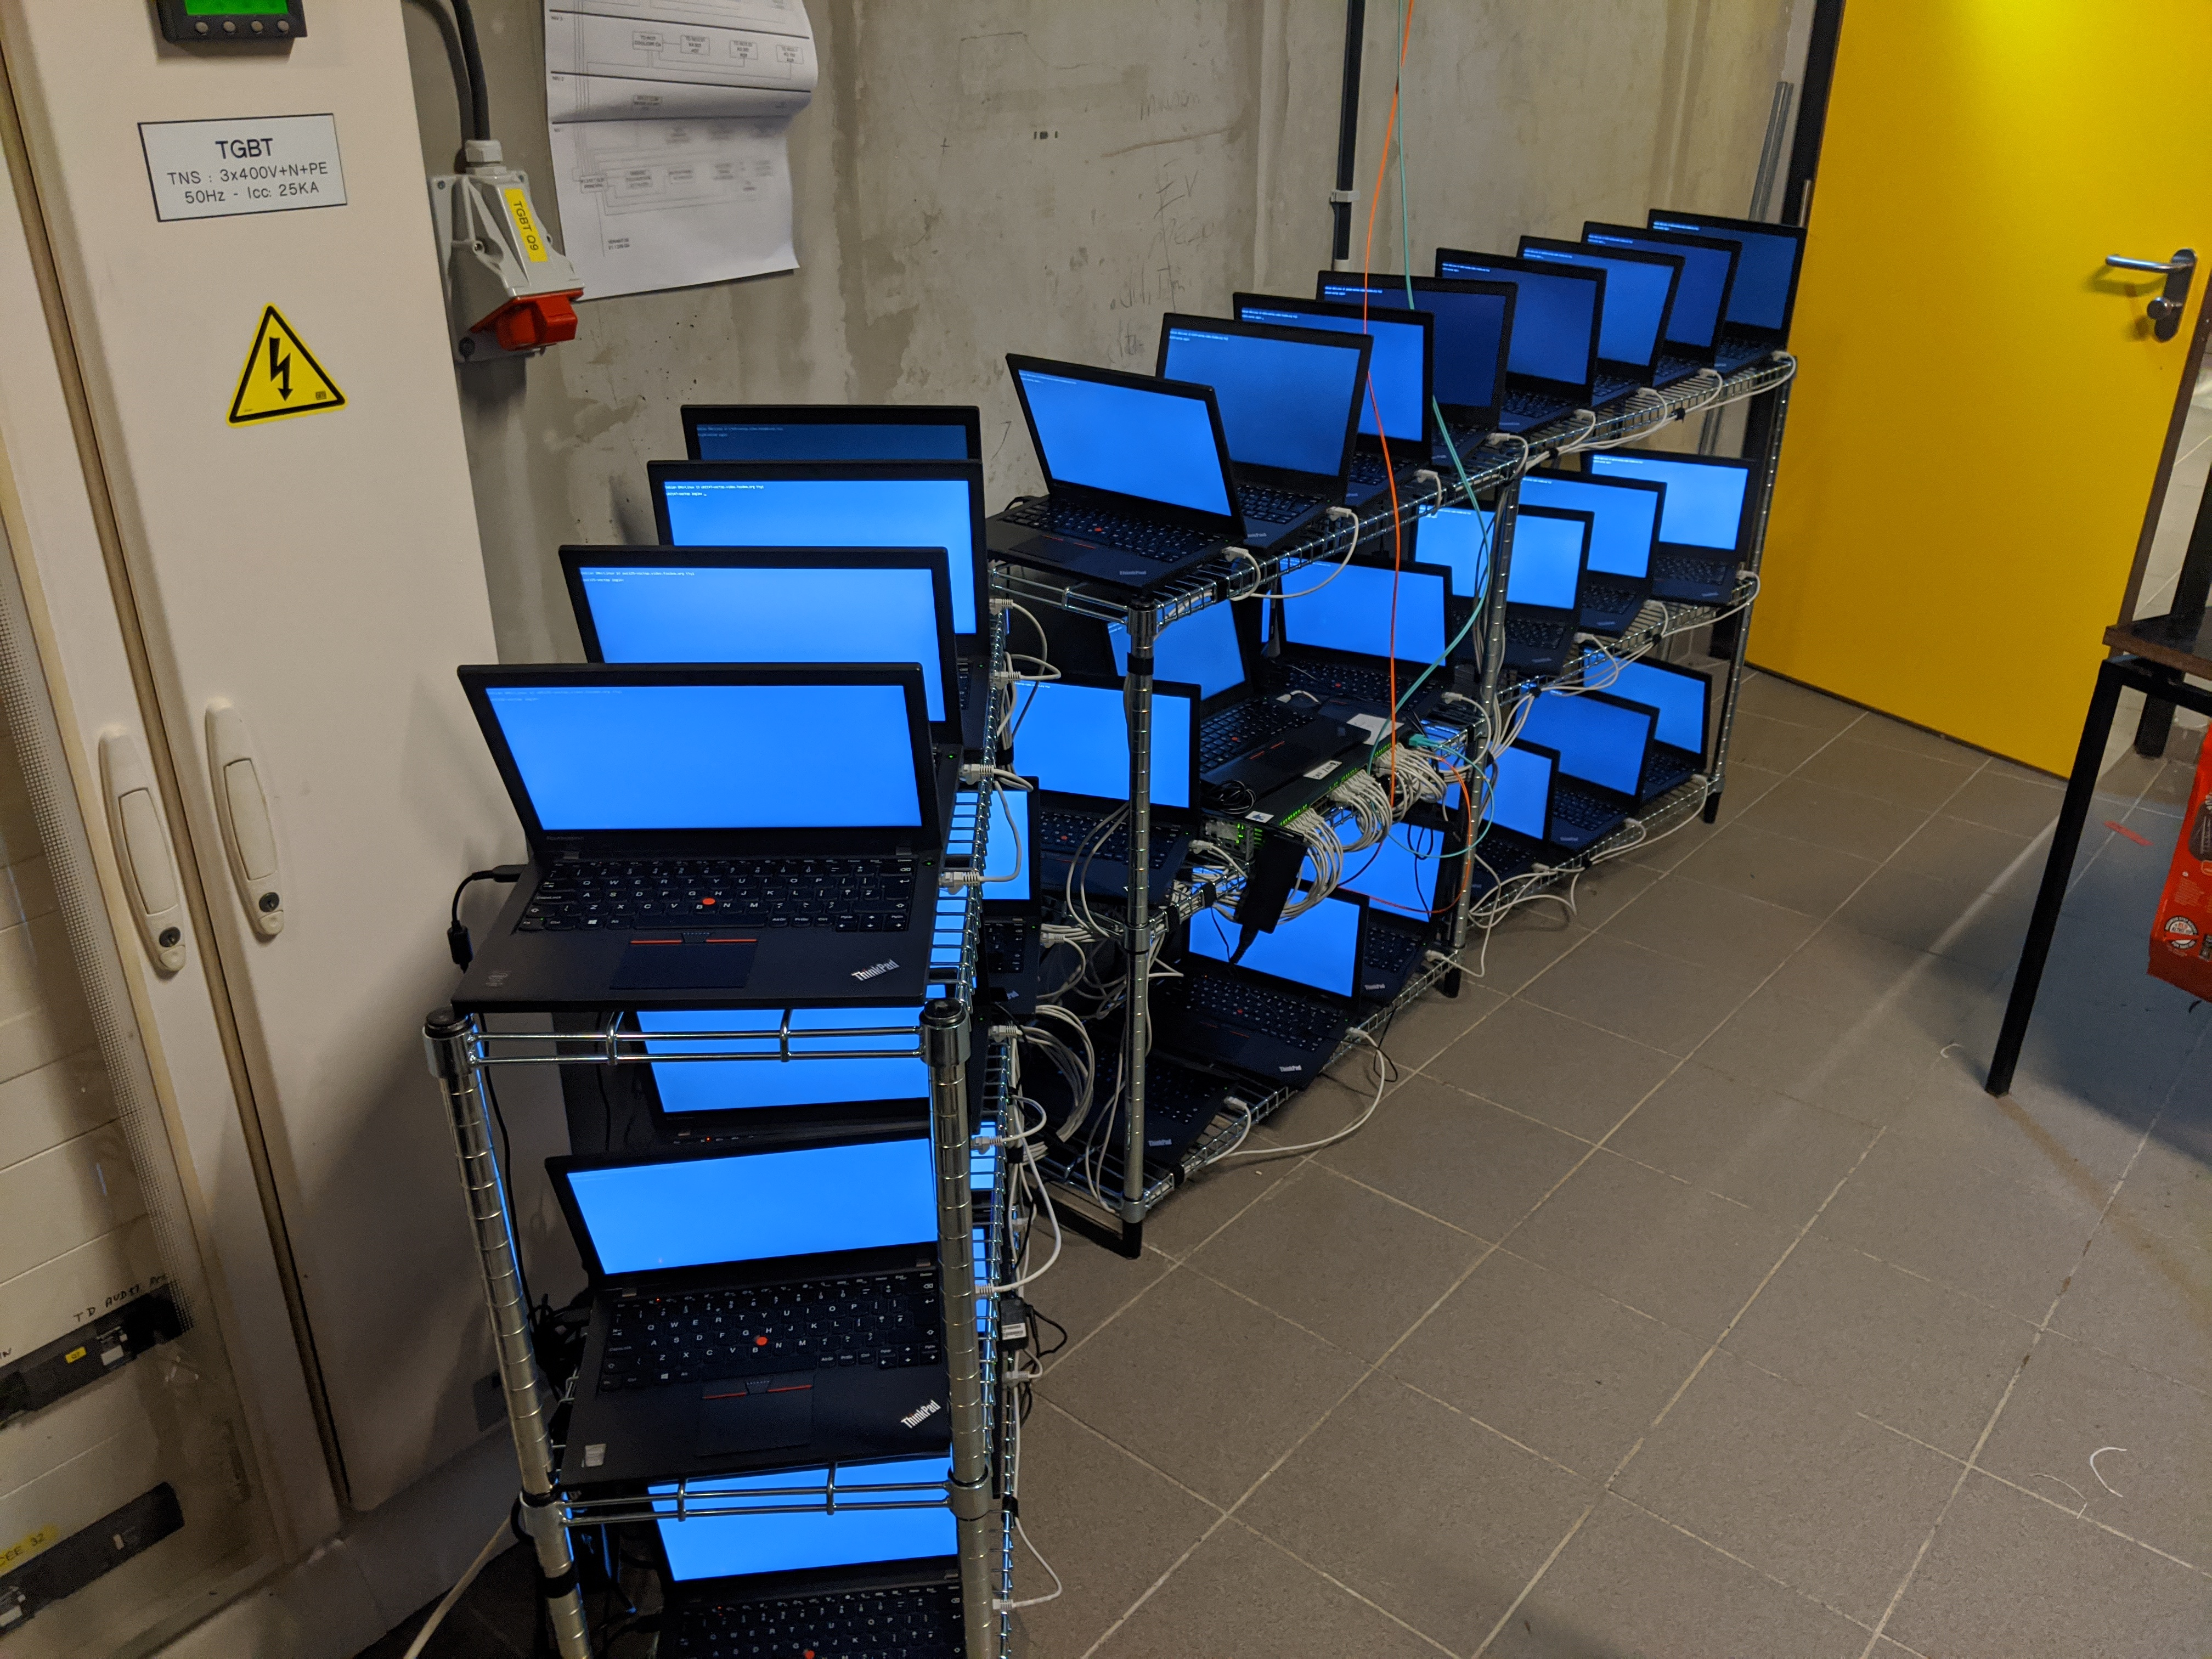
\includegraphics[width=80mm]{render_farm.jpg}
	\end{figure}
	\vfill
\end{frame}

\begin{frame}
	\frametitle{DNS64}
	\vfill
	\begin{itemize}
		\item The last few years, we ran DNS64 on Bind
		\item This year, it's CoreDNS
		\item 50\% reduction in CPU usage
	\end{itemize}
	\vfill
\end{frame}

\begin{frame}
	\frametitle{Timelines}
	\vfill
	\begin{itemize}
		\item Installation of router
		\begin{itemize}
			\item 2016: Friday
			\item 2017: December
			\item 2018: December
			\item 2019: December
			\item 2020: December
		\end{itemize}
		\item Network up
		\begin{itemize}
			\item 2015: Saturday 05:00
			\item 2016: Friday 19:00
			\item 2017: Friday 16:00
			\item 2018: Friday 12:00
			\item 2019: Thursday, last hiccups solved on Friday 19:00
			\item 2020: Friday 18:00
		\end{itemize}
	\end{itemize}
	\vfill
\end{frame}

\begin{frame}
	\frametitle{Timelines}
	\begin{itemize}
	\vfill
		\item Monitoring
		\begin{itemize}
			\item 2016: Saturday 12:00
			\item 2017: Saturday 09:00
			\item 2018: January
			\item 2019: January
			\item 2020: January 2019! :)
		\end{itemize}
		\item Video
		\begin{itemize}
			\item 2016: Saturday 11:30
			\item 2017: Saturday 09:30
			\item 2018: Saturday 08:30
			\item 2019: Friday 21:00
			\item 2020: Friday 19:00
		\end{itemize}
	\end{itemize}
	\vfill
\end{frame}


\begin{frame}
	\frametitle{Next year}
	\vfill
	Centralized syslog for all teams through Loki
	\vfill
\end{frame}


\begin{frame}
	\frametitle{Clone our conference}
	\vfill
	\begin{itemize}
		\item Try our monitoring: \\ \url{https://dashboard.fosdem.org}
		\item Clone our conference: \\ \url{https://github.com/FOSDEM/infrastructure}
		\item We might be able to start helping other conferences. Ongoing dicussions and we hope to be able to do that
	\end{itemize}
	\vfill
\end{frame}


\end{document}

%\begin{frame}
%	\frametitle{}
%	\begin{itemize}
%		\item 
%		\item 
%		\item 
%		\item 
%		\item 
%	\end{itemize}
%\end{frame}
